\renewcommand{\NomeBloco}{APS\_3}
\renewcommand{\NomeBlocoNoUnderline}{apsthree}
\renewcommand{\NomePTab}{tab_\NomeBlocoNoUnderline}
\renewcommand{\NomeSTab}{tab_\NomeBlocoNoUnderline2}
\renewcommand{\NomePFig}{fig_\NomeBlocoNoUnderline}
\renewcommand{\NomeSFig}{fig_\NomeBlocoNoUnderline2}
\renewcommand{\NomeTTab}{tab_\NomeBlocoNoUnderline3}
\renewcommand{\NomeQTab}{tab_\NomeBlocoNoUnderline4}

\section{\NomeBloco}

O \emph{\NomeBloco} \'e o circuito respons\'avel por armazenar todos os tr\^es blocos APS de cor (Azul, Verde, Vermelho), mais o TIA geradora de rel\'ogio de refer\^encia para os APS's citados. O bloco apresenta as defini{\c c}\~oes de sinais de entrada e sa\'ida referidos na \autoref{\NomeSTab}.

\begin{table}[htb]
\centering
\IBGEtab{%
  \caption{Descri{\c c}\~ao dos sinais de entrada e sa\'ida do circuito projetado para as cores azul, verde e vermelha}%
  \label{\NomeSTab}
}{%
  \begin{tabular}{ccll}
  \toprule
   Sinal & Tipo & Descri{\c c}\~ao & Observa{\c c}\~ao \\
  \midrule \midrule
   RESET\_BLUE & Entrada & \begin{tabular}[c]{@{}c@{}}Sinal de \emph{RESET} no APS\\ para cor azul\end{tabular} & Ativo em n\'ivel baixo \\
  \midrule
   RESET\_GREEN & Entrada & \begin{tabular}[c]{@{}c@{}}Sinal de \emph{RESET} no APS\\ para cor verde\end{tabular} & Ativo em n\'ivel baixo \\
  \midrule
   RESET\_RED & Entrada & \begin{tabular}[c]{@{}c@{}}Sinal de \emph{RESET} no APS\\ para cor vermelha\end{tabular} & Ativo em n\'ivel baixo \\
   \midrule
   ENABLE\_BLUE & Entrada & \begin{tabular}[c]{@{}c@{}}Sinal de \emph{ENABLE} no APS\\ para cor azul\end{tabular} & Ativo em n\'ivel alto \\
  \midrule
   ENABLE\_GREEN & Entrada & \begin{tabular}[c]{@{}c@{}}Sinal de \emph{ENABLE} no APS\\ para cor verde\end{tabular} & Ativo em n\'ivel alto \\
  \midrule
   ENABLE\_RED & Entrada & \begin{tabular}[c]{@{}c@{}}Sinal de \emph{ENABLE} no APS\\ para cor vermelha\end{tabular} & Ativo em n\'ivel alto \\
  \midrule
   Ibias\_comp1 & Entrada & Fonte de corrente para cor Azul &  \\
   \midrule
   Ibias\_comp2 & Entrada & Fonte de corrente para cor Verde &  \\
   \midrule
   Ibias\_comp3 & Entrada & Fonte de corrente para cor Vermelha &  \\
   \midrule
   Ibias\_clk & Entrada & \begin{tabular}[c]{@{}c@{}}Fonte de corrente para o bloco\\ \emph{APS\_pixel\_clk}\end{tabular}
    &  \\
  \midrule
   Out\_An\_Blue & Sa\'ida & Sinal anal\'ogico para cor azul \\
  \midrule
   Out\_Dig\_Blue & Sa\'ida & Sinal digital para cor azul \\
  \midrule
   Out\_An\_Green & Sa\'ida & Sinal anal\'ogico para cor verde \\
  \midrule
   Out\_Dig\_Green & Sa\'ida & Sinal digital para cor verde \\
  \midrule
   Out\_An\_Red & Sa\'ida & Sinal anal\'ogico para cor vermelha \\
  \midrule
   Out\_Dig\_Red & Sa\'ida & Sinal digital para cor vermelha \\
  \bottomrule
\end{tabular}%
}{%
  \fonte{Produzido pelo autor.}
}
\end{table}

O circuito projetado para o bloco \'e demonstrado na \autoref{\NomePFig}.

\begin{figure}[htb]
 \label{\NomePFig}
 \centering
    \centering
    \caption{Circuito CMOS projetado para o bloco \NomeBloco} 
    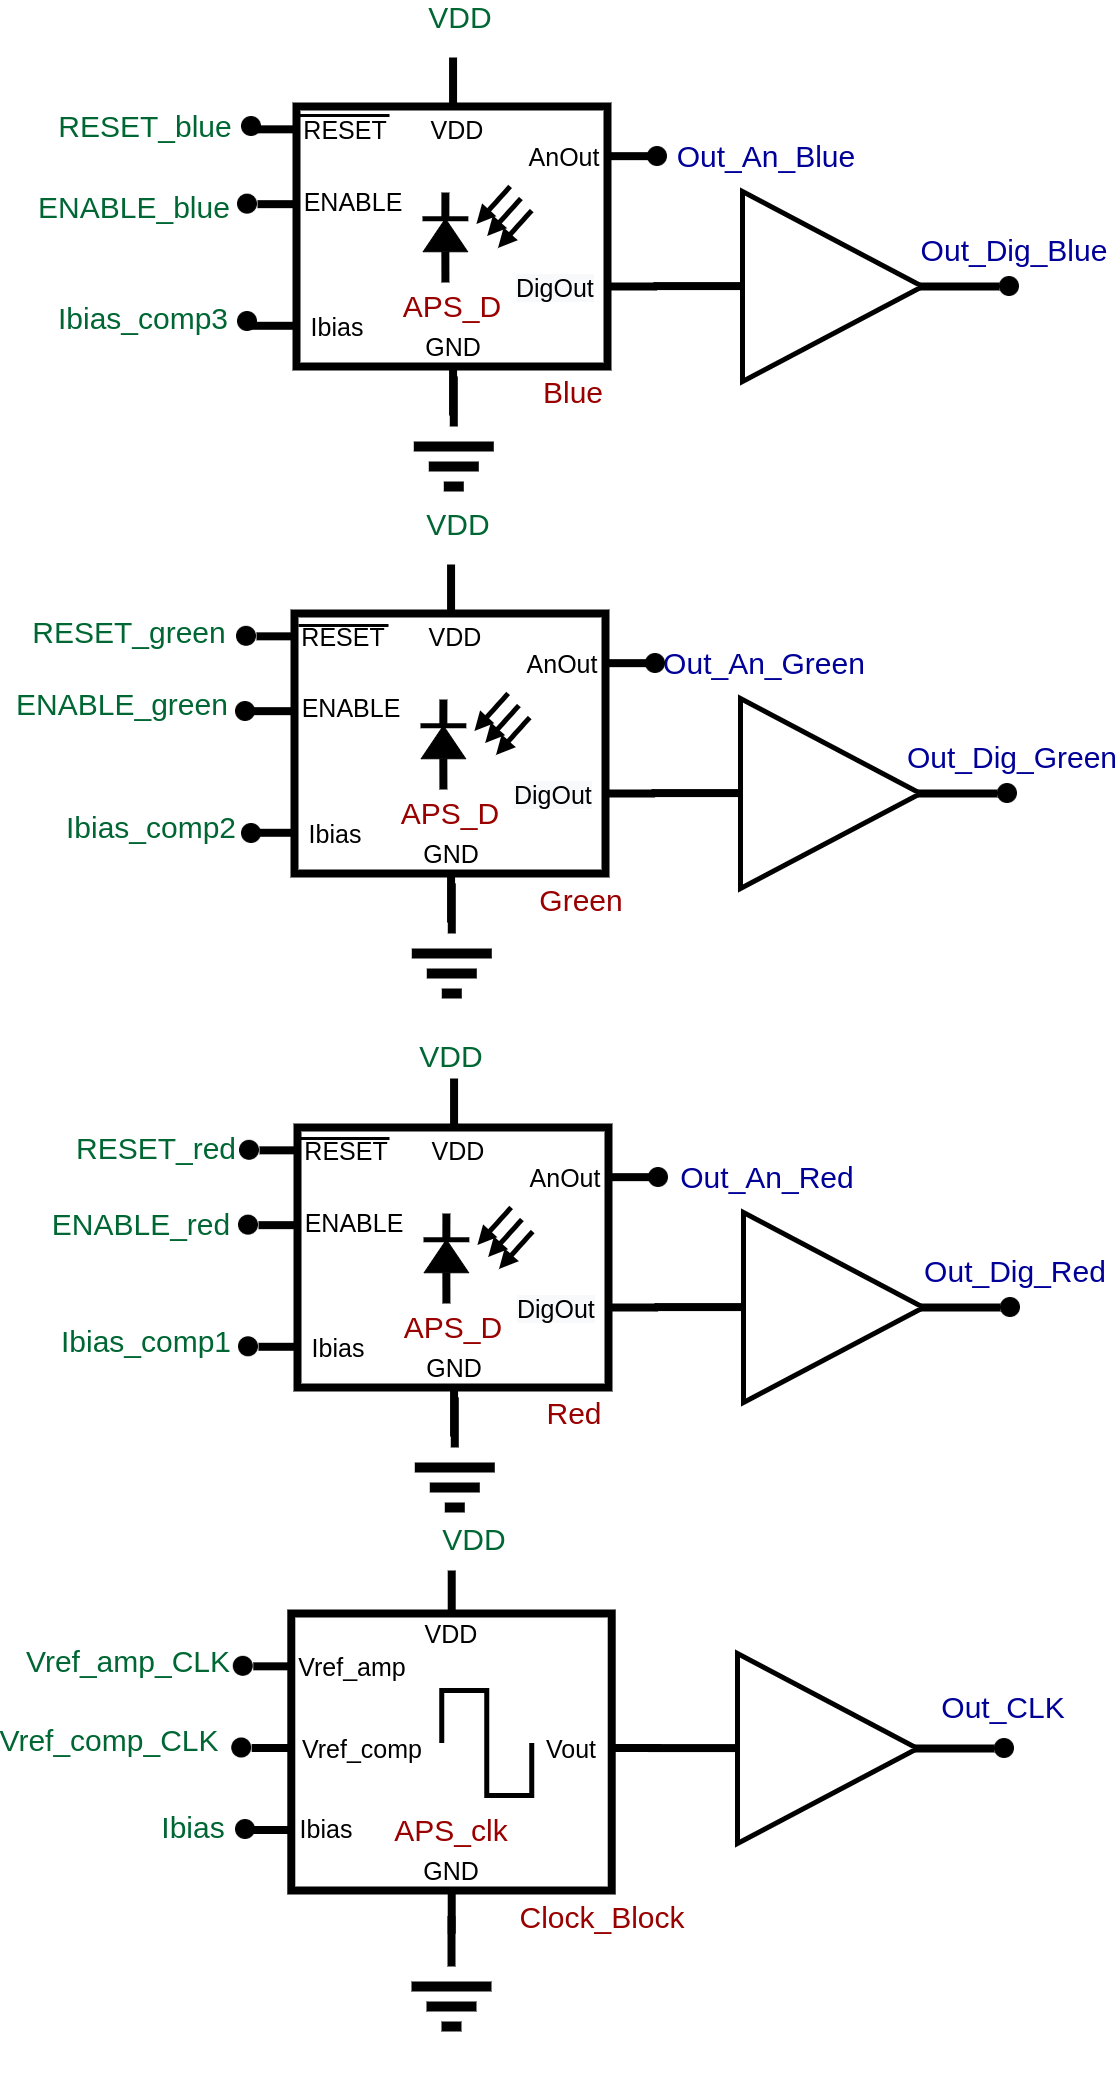
\includegraphics[scale=0.3]{Circuitos/APS_3.png}
    \legend{Fonte: Produzido pelo autor}
\end{figure}

\begin{figure}[htb]
 \centering
    \centering
    \caption{Representa{\c c}\~ao em bloco do \NomeBloco} \label{\NomeSFig}
    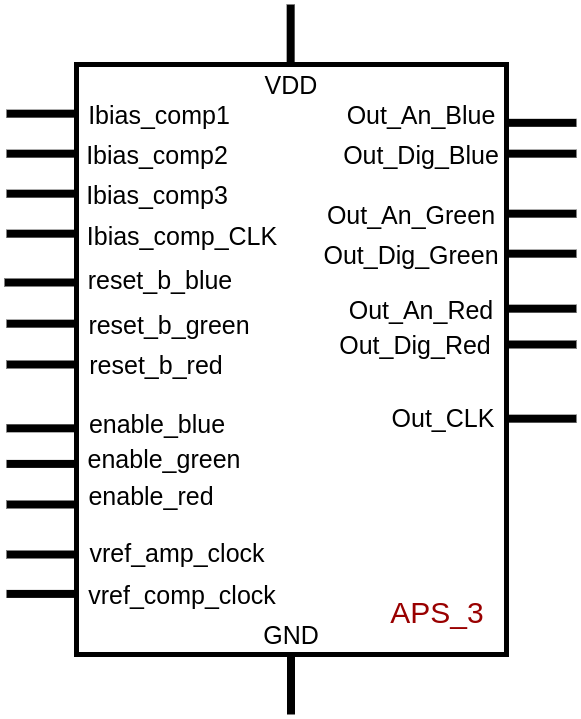
\includegraphics[scale=0.3]{Circuitos/APS_3_block.png}
    \legend{Fonte: Produzido pelo autor}
\end{figure}

As sa\'idas digitais de cada bloco APS\_digitalized apresentam um buffer, de forma a garantir a integridade do sinal nos pinos do Circuito Integrado.
\clearpage